\documentclass[a4paper,11pt]{report}
\usepackage[showexo=true,showcorr=false]{../packages/coursclasse}

% - Fraction d'un tout
% - Pourcentages
% - Calculer le pourcentage d'un tout 

%Commenter ou enlever le commentaire sur la ligne suivante pour montrer le niveau
\toggletrue{montrerNiveaux}
%permet de gérer l'espacement entre les items des env enumerate et enumitem
\usepackage{enumitem}
\setlist[enumerate]{align=left,leftmargin=1cm,itemsep=10pt,parsep=0pt,topsep=0pt,rightmargin=0.5cm}
\setlist[itemize]{align=left,labelsep=1em,leftmargin=*,itemsep=0pt,parsep=0pt,topsep=0pt,rightmargin=0cm}
%permet de gerer l'espacement entre les colonnes de multicols
\setlength\columnsep{35pt}


\begin{document}
%%%%%%%%%%%%%%%%% À MODIFIER POUR CHAQUE SERIE %%%%%%%%%%%%%%%%%%%%%%%%%%%%%
\newcommand{\chapterName}{Nombres et opérations}
\newcommand{\serieName}{Partie d'un tout et pourcentages}


%%%%%%%%%%%%%%%%%% PREMIERE PAGE NE PAS MODIFER %%%%%%%%%%%%%%%%%%%%%%%%
% le chapitre en cours, ne pas changer au cours d'une série
\chapter*{\chapterName}
\thispagestyle{empty}

%%%%% LISTE AIDE MEMOIRE %%%%%%
\begin{amL}{\serieName}{
	\item Calculer la fraction d'un nombre (page 31)
	\item Définition d'un pourcentage (page 58)
	\item Déterminer un pourcentage (page 58)
}
\end{amL}

%%%%%%%%%%%%%%% DEBUT DE LA SERIE NE PAS MODIFIER %%%%%%%%%%%%%%%%%%%%%%%%%%%%%
\section*{\serieName}
\setcounter{page}{1}
\thispagestyle{firstPage}



%%%%%%%%%%% LES EXERCICES %%%%%%%%%%%%%%%%%%%%%%%%%%%%%%%%%%%

\begin{resolu}{Calculer la partie d'un tout}{
Calcule. 


\begin{tasks}(1)
	\task $\dfrac{1}{5}$ de \tunit{8,50}{\fr}


On présente deux méthodes. La première méthode juste avec des calculs et la seconde avec une représentation graphique. 
	Méthode 1: $\dfrac{1}{5}$ de \tunit{8,50}{\fr}
	$=\dfrac{1}{5}\cdot 8,50=1\cdot 8,50 \div 5=\tunit{1,70}{\fr}$

	Méthode 2: \tunit{8,50}{\fr} représente le tout, c'est-à-dire les cinq parts
\scalebox{1}{
		\begin{tikzpicture}
  %\node at (-1/2,0) {$\ldots\ldots\ldots$};
  \pic  at (0, 0) {circle fraction={5/5}};
\end{tikzpicture}}.
On souhaite déterminer la valeur de $\dfrac{1}{5}$, donc une part
\scalebox{1}{
		\begin{tikzpicture}
  %\node at (-1/2,0) {$\ldots\ldots\ldots$};
  \pic  at (0, 0) {circle fraction={1/5}};
\end{tikzpicture}}. Pour cela, on divise \tunit{8,50}{\fr} par cinq (pour déterminer à combien correspond une part). On obtient ainsi la valeur de $\dfrac{1}{5}$ de \tunit{8,50}{\fr}

\task $\dfrac{3}{4}$ de \tunit{1,2}{\m}

Méthode 1: $\dfrac{3}{4}$ de \tunit{1,2}{\m} $=\dfrac{3}{4}\cdot 1,2=3\cdot 1,2\div 4=\tunit{0,9}{\m}$

Méthode 2: \tunit{1,2}{\m} représente le tout, c'est-à-dire les quatre parts
\scalebox{1}{
		\begin{tikzpicture}
  %\node at (-1/2,0) {$\ldots\ldots\ldots$};
  \pic  at (0, 0) {circle fraction={4/4}};
\end{tikzpicture}}.
On souhaite déterminer la valeur de $\dfrac{3}{4}$, donc de 3 parts
\scalebox{1}{
		\begin{tikzpicture}
  %\node at (-1/2,0) {$\ldots\ldots\ldots$};
  \pic  at (0, 0) {circle fraction={3/4}};
\end{tikzpicture}}. Pour cela, on divise \tunit{1,2}{\m} par quatre (pour déterminer à combien correspond une part). On en prend ensuite trois (on multiplie le résultat obtenu par trois). On obtient ainsi la valeur de $\dfrac{3}{4}$ de $1,2$ $m$.
\task $\dfrac{1}{5}$ de \tunit{68}{\fr}$=\dfrac{1}{5}\cdot 68=1\cdot 68\div 5=\tunit{13,6}{\m}$
\task $\dfrac{8}{5}$ de $145$ $\ell=\dfrac{8}{5}\cdot 145=8\cdot 145\div 5=232$ $\ell$
\end{tasks}
}{1}
\end{resolu}

\begin{exo}{
Calcule.
\begin{tasks}(3)
	\task $\dfrac{1}{4}$ de \tunit{7,20}{\fr}
	\task $\dfrac{1}{8}$ de \tunit{5,6}{\m}
	\task $\dfrac{1}{5}$ de \tunit{68}{\fr}
	\task $\dfrac{1}{5}$ de \tunit{145}{\l}
	\task $\dfrac{1}{3}$ de \tunit{8,40}{\fr}
	\task $\dfrac{1}{4}$ de \tunit{78}{\fr}
	\task $\dfrac{1}{6}$ de \tunit{16,2}{\m}
	\task $\dfrac{1}{2}$ de \tunit{9,60}{\m}
\end{tasks}
 \vspace{1pt}
}{1}\end{exo}

\begin{exo}{
Calcule.
\begin{tasks}(3)
	\task les $\dfrac{2}{3}$ de \tunit{28,80}{\fr}
	\task les $\dfrac{3}{5}$ de \tunit{176}{\fr}
	\task les $\dfrac{3}{4}$ de \tunit{88}{\m}
	\task les $\dfrac{2}{3}$ de \tunit{378}{\m^2}
	\task les $\dfrac{2}{5}$ de \tunit{72}{\l}
	\task les $\dfrac{4}{5}$ de \tunit{12,50}{\fr}
	\task les $\dfrac{3}{8}$ de \tunit{144}{\fr}
	\task les $\dfrac{3}{10}$ de \tunit{78}{\fr}
\end{tasks}
 \vspace{1pt}
}{1}\end{exo}

\begin{exo}{
Calcule.
\begin{tasks}(3)
	\task $\dfrac{1}{4}$ de \tunit{18,40}{\fr}
	\task $\dfrac{3}{5}$ de \tunit{43}{\m}
	\task $\dfrac{2}{3}$ de \tunit{126}{\m^2}
	\task $\dfrac{5}{6}$ de \tunit{22,8}{\fr}
	\task $\dfrac{3}{4}$ de \tunit{48,8}{\l}
	\task $\dfrac{4}{7}$ de \tunit{294}{\fr}
	\task $\dfrac{7}{10}$ de \tunit{68}{\fr}
	\task $\dfrac{3}{4}$ de \tunit{64}{\m^2}
\end{tasks}
 \vspace{1pt}
}{1}\end{exo}

\begin{exol}{NO208}{55}{1}
\end{exol}
\begin{exol}{NO206}{54}{1}
\end{exol}
\begin{exol}{NO207}{54}{1}
\end{exol}
\begin{exol}{NO209}{55}{1}
\end{exol}
\begin{exol}{NO210}{55}{1}
\end{exol}
\begin{exol}{NO211}{55}{1}
\end{exol}
\begin{exol}{NO214}{56}{1}
\end{exol}

\begin{resolu}{Sous forme de pourcentage}{
	Écris les nombres suivants sous forme de pourcentage.

	{\color{blue} Un pourcentage est une fraction dont le dénominateur vaut $100$. Voici la procédure à suivre:
	\begin{tasks}(1)
		\task[1.] Écrire le nombre sous forme de fraction (si ce n'est pas déjà fait).
		\task[2.] Amplifier ou simplifier la fraction afin d'obtenir un dénominateur égal à $100$. 
\end{tasks}
}
\begin{tasks}(1)
	\task $\dfrac{5}{25}=\dfrac{5\cdot 4}{25\cdot 4}=\dfrac{20}{100}=20\%.$
	\task $0,1=\dfrac{1}{10}=\dfrac{1\cdot 10}{10\cdot 10}=\dfrac{10}{100}=10\%.$
	\task $\dfrac{3}{50}=\dfrac{3\cdot 2}{50\cdot 2}=\dfrac{6}{100}=6\%.$
\end{tasks}}{1}
\end{resolu}

\begin{exo}{
Écris sous forme d'un pourcentage.
	\begin{tasks}(6)
	\task $0,3$
	\task $1,4$
	\task $\dfrac{3}{4}$
	\task $\dfrac{5}{2}$
	\task $\dfrac{7}{10}$
	\task $\dfrac{3}{20}$
	\end{tasks}
 \vspace{1pt}
}{1}\end{exo}

\begin{exo}{
Écris sous forme d'un pourcentage.
	\begin{tasks}(6)
	\task $2,5$
	\task $0,25$
	\task $0,65$
	\task $1$
	\task $\dfrac{80}{10}$
	\task $\dfrac{8}{5}$
	\end{tasks}
 \vspace{1pt}
}{1}\end{exo}

\begin{exo}{
Écris sous forme d'un pourcentage lorsque cela est possible.
\begin{tasks}(3)
\task $2,3$
\task $0,4$
\task $\dfrac{8}{50}$
\task $\dfrac{4}{9}$
\task $\dfrac{3}{25}$
\task $\dfrac{120}{500}$
\task $\dfrac{15}{300}$
\task $\dfrac{5}{40}$
\task $\dfrac{25}{200}$
\end{tasks}
 \vspace{1pt}
}{2}\end{exo}

\begin{exo}{
Écris les pourcentages suivants sous forme de fractions irréductibles.
\begin{tasks}(3)
\task $10\%$
\task $18\%$
\task $150\%$
\task $45\%$
\task $65\%$
\task $30\%$
\end{tasks}
 \vspace{1pt}
}{1}\end{exo}

\begin{exo}{
Écris les pourcentages suivants sous forme de fractions irréductibles.
\begin{tasks}(3)
\task $5\%$
\task $20\%$
\task $63\%$
\task $78\%$
\task $210\%$
\task $300\%$
\end{tasks}
 \vspace{1pt}
}{2}\end{exo}

\begin{qmoodle}{Pourcentage}{4}{
	\begin{center}	
		Q1


\includegraphics[scale=1]{media/qr/ptpq1}

\tiny{{https://edu.ge.ch/qr/ptpq1}}
\end{center}
	\begin{center}	
		Q2


\includegraphics[scale=1]{media/qr/ptpq2}

\tiny{{https://edu.ge.ch/qr/ptpq2}}
\end{center}
	\begin{center}	
		Q3


\includegraphics[scale=1]{media/qr/ptpq3}

\tiny{{https://edu.ge.ch/qr/ptpq3}}
\end{center}
\begin{center}	
		Q4

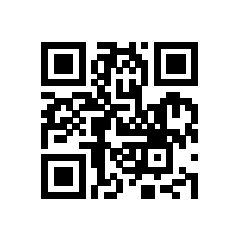
\includegraphics[scale=1]{media/qr/ptpq4}

\tiny{{https://edu.ge.ch/qr/ptpq4}}
\end{center}
}
\end{qmoodle}

\begin{exo}{
	Calcule.
		\begin{tasks}(3)
			\task $30\%$ de \tunit{40}{\kg}
			\task $25\%$ de \tunit{160}{\fr} 
			\task $45\%$ de \tunit{20}{\g}
			\task $120\%$ de \tunit{75}{\fr} 
			\task $100\%$ de \tunit{34}{\kg} 
			\task $30\%$ de \tunit{30}{\fr} 
	\end{tasks}
 \vspace{1pt}
}{1}\end{exo}


\begin{exo}{
	Calcule.
		\begin{tasks}(3)
			\task $24\%$ de \tunit{35}{\fr}
			\task $58\%$ de \tunit{10}{\fr} 
			\task $152\%$ de \tunit{1000}{\kg}
		\task $77\%$ de \tunit{41}{\l} 
		\task $600\%$ de \tunit{12}{\fr}
		\task $43\%$ de \tunit{70}{\kg} 
	\end{tasks}
 \vspace{1pt}
}{2}\end{exo}

\begin{qmoodle}{Partie d'un tout}{2}{
	\begin{center}	
		Q1


\includegraphics[scale=1]{media/qr/ptpq5}

\tiny{{https://edu.ge.ch/qr/ptpq5}}
\end{center}
	\begin{center}	
		Q2

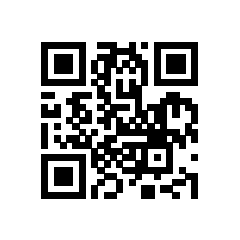
\includegraphics[scale=1]{media/qr/ptpq6}

\tiny{{https://edu.ge.ch/qr/ptpq6}}
\end{center}
}
\end{qmoodle}
\section*{Retrouver le tout}
\begin{resolu}{Retrouver un tout}{

On présente deux méthodes. La première méthode juste avec des calculs et la seconde avec une représentation graphique. 

Retrouve le tout si
\begin{tasks}[after-item-skip = 0.3em, after-skip=-0.5em](1)
	\task $\dfrac{1}{7}$ vaut $11$. 

		Méthode 1: Pour retrouver le tout, on divise la partie (ici $11$) par le numérateur de la fraction (ici $1$) puis on multiplie par le dénominateur de la fraction (ici $7$). On obtient que le tout vaut $11\div 1\cdot 7=77$.

	Méthode 2:	$\dfrac{1}{7}$ vaut $11$, donc une part vaut $11$ 
\scalebox{1}{
		\begin{tikzpicture}
  %\node at (-1/2,0) {$\ldots\ldots\ldots$};
  \pic  at (0, 0) {circle fraction={1/7}};
\end{tikzpicture}}. La question est combien vaut l'entier, c'est-à-dire les sept parts 
\scalebox{1}{
		\begin{tikzpicture}
  %\node at (-1/2,0) {$\ldots\ldots\ldots$};
  \pic  at (0, 0) {circle fraction={7/7}};
\end{tikzpicture}}? Si une part vaut $11$, alors sept parts valent $7\cdot 11=77$. 

	\task $\dfrac{3}{13}$ vaut $9$. 

		Méthode 1: Le tout vaut $9\div 3\cdot 13=39$.
		
		Méthode 2: $\dfrac{3}{13}$ vaut $9$, donc trois parts valent $9$ 
\scalebox{1}{
		\begin{tikzpicture}
  %\node at (-1/2,0) {$\ldots\ldots\ldots$};
  \pic  at (0, 0) {circle fraction={3/13}};
\end{tikzpicture}}. La question est combien vaut l'entier, c'est-à-dire les treize parts 
\scalebox{1}{
		\begin{tikzpicture}
  %\node at (-1/2,0) {$\ldots\ldots\ldots$};
  \pic  at (0, 0) {circle fraction={13/13}};
\end{tikzpicture}}? Si trois parts valent $9$, alors une part vaut $9\div 3=3$ et les treize parts valent $3\cdot 13=39$. 

	\task $\dfrac{4}{5}$ vaut $16$. Le tout vaut $16\div 4\cdot 5=20$.
	\task $\dfrac{2}{7}$ vaut $10$. Le tout vaut $10\div 2 \cdot 7=35$.
	\task $\dfrac{8}{9}$ vaut $72$. Le tout vaut $72\div 8\cdot 9=81$.
	\task $\dfrac{6}{10}$ vaut $30$. Le tout vaut $30\div 6\cdot 10=50.$
\end{tasks}
}{1}\end{resolu}
\begin{exo}{
Retrouve le tout si
	\begin{tasks}(3)
	\task $\dfrac{1}{5}$ vaut $3$
	\task $\dfrac{3}{7}$ vaut $12$
	\task $\dfrac{1}{3}$ vaut $11$
	\task $\dfrac{3}{4}$ vaut $15$
	\task $\dfrac{11}{20}$ vaut $22$
	\task $\dfrac{14}{16}$ vaut $42$
	\end{tasks}
}{1}\end{exo}
\begin{exo}{
Retrouve le tout si
	\begin{tasks}(3)
	\task $\dfrac{14}{20}$ vaut $7$
	\task $\dfrac{30}{56}$ vaut $6$
	\task $\dfrac{12}{25}$ vaut $3$
	\task $\dfrac{7}{3}$ vaut $14$
	\task $\dfrac{24}{50}$ vaut $9$
	\task $\dfrac{15}{17}$ vaut $1,5$
	\end{tasks}
}{2}\end{exo}
\begin{exo}{
Retrouve le tout si
	\begin{tasks}(2)
	\task $90\%$ vaut $18$
	\task $85\%$ vaut $4,25$
	\task $45\%$ vaut $9,9$
	\task $20\%$ vaut $1,2$
	\task $65\%$ vaut $6,76$
	\task $72\%$ vaut $9$
	\end{tasks}
}{1}\end{exo}

\begin{exo}{
Retrouve le tout si
	\begin{tasks}(2)
	\task $95\%$ vaut $47,5$
	\task $42\%$ vaut $85,26$
	\task $63\%$ vaut $25,2$
	\task $5\%$ vaut $1,75$
	\task $15\%$ vaut $75$
	\task $20\%$ vaut $14,5$
	\end{tasks}
}{2}\end{exo}
\begin{exo}{
Retrouve le tout si
	\begin{tasks}(2)
	\task $38\%$ vaut $11,4$
	\task $70\%$ vaut $14$
	\task $82\%$ vaut $5,74$
	\task $99\%$ vaut $4,95$
	\task $7\%$ vaut $28$
	\task $3\%$ vaut $45,6$
	\end{tasks}
}{2}\end{exo}

\begin{qmoodle}{Retrouver le tout}{2}{
	\begin{center}	
		Q1

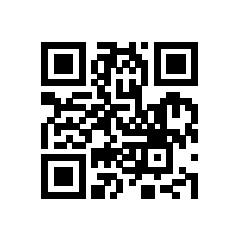
\includegraphics[scale=1]{media/qr/ptpq7}

\tiny{{https://edu.ge.ch/qr/ptpq7}}
\end{center}
	\begin{center}	
		Q2


\includegraphics[scale=1]{media/qr/ptpq8}

\tiny{{https://edu.ge.ch/qr/ptpq8}}
\end{center}
}
\end{qmoodle}


%\exof{NO202}{70}{2}
%\exol{NO212}{55}{1}
%\exol{NO213}{56}{1}










\end{document}
